\documentclass[11pt]{report}
\usepackage{titlesec}
\titleformat{\chapter}
{\filcenter\normalfont\Large\bfseries}
{\chaptertitlename~\thechapter} {0.5em} {}

\usepackage[dutch]{babel}
\usepackage{graphicx}
\usepackage{amsmath,amssymb}
\usepackage{bbm}
\usepackage{listings} %listing R code
\usepackage{siunitx} %voor 10^
\usepackage[usenames,dvipsnames]{color}
\usepackage{color}
\usepackage{enumitem}
\usepackage{pdfpages}
\usepackage{titling}
\usepackage{hyperref}

\usepackage{amssymb}

\usepackage[T1]{fontenc}
\usepackage[utf8]{inputenc}
\usepackage{charter}
\usepackage{environ}
\usepackage{tikz}
\usetikzlibrary{calc,matrix}

%%%%%%%%%%%%%%%%%%%%%%%%%%%%%%%%
% code by Andrew:
% http://tex.stackexchange.com/a/28452/13304
\makeatletter
\let\matamp=&
\catcode`\&=13
\makeatletter
\def&{\iftikz@is@matrix
  \pgfmatrixnextcell
  \else
  \matamp
  \fi}
\makeatother

\newcounter{lines}
\def\endlr{\stepcounter{lines}\\}

\newcounter{vtml}
\setcounter{vtml}{0}

\newif\ifvtimelinetitle
\newif\ifvtimebottomline
\tikzset{description/.style={
  column 2/.append style={#1}
 },
 timeline color/.store in=\vtmlcolor,
 timeline color=red!80!black,
 timeline color st/.style={fill=\vtmlcolor,draw=\vtmlcolor},
 use timeline header/.is if=vtimelinetitle,
 use timeline header=false,
 add bottom line/.is if=vtimebottomline,
 add bottom line=false,
 timeline title/.store in=\vtimelinetitle,
 timeline title={},
 line offset/.store in=\lineoffset,
 line offset=4pt,
}

\NewEnviron{vtimeline}[1][]{%
\setcounter{lines}{1}%
\stepcounter{vtml}%
\begin{tikzpicture}[column 1/.style={anchor=east},
 column 2/.style={anchor=west},
 text depth=0pt,text height=1ex,
 row sep=1ex,
 column sep=1em,
 #1
]
\matrix(vtimeline\thevtml)[matrix of nodes]{\BODY};
\pgfmathtruncatemacro\endmtx{\thelines-1}
\path[timeline color st] 
($(vtimeline\thevtml-1-1.north east)!0.5!(vtimeline\thevtml-1-2.north west)$)--
($(vtimeline\thevtml-\endmtx-1.south east)!0.5!(vtimeline\thevtml-\endmtx-2.south west)$);
\foreach \x in {1,...,\endmtx}{
 \node[circle,timeline color st, inner sep=0.15pt, draw=white, thick] 
 (vtimeline\thevtml-c-\x) at 
 ($(vtimeline\thevtml-\x-1.east)!0.5!(vtimeline\thevtml-\x-2.west)$){};
 \draw[timeline color st](vtimeline\thevtml-c-\x.west)--++(-3pt,0);
 }
 \ifvtimelinetitle%
  \draw[timeline color st]([yshift=\lineoffset]vtimeline\thevtml.north west)--
  ([yshift=\lineoffset]vtimeline\thevtml.north east);
  \node[anchor=west,yshift=16pt,font=\large]
   at (vtimeline\thevtml-1-1.north west) 
   {\textsc{Timeline \thevtml}: \textit{\vtimelinetitle}};
 \else%
  \relax%
 \fi%
 \ifvtimebottomline%
   \draw[timeline color st]([yshift=-\lineoffset]vtimeline\thevtml.south west)--
  ([yshift=-\lineoffset]vtimeline\thevtml.south east);
 \else%
   \relax%
 \fi%
\end{tikzpicture}
}
%%%%%%%%%%%%%%%%%%%%%%%%%%%%%%%%

\newcommand{\half}{\frac{1}{2}}
\newcommand{\pref}[1]{(\ref{#1})}
\newcommand{\itab}[1]{\hspace{0em}\rlap{#1}}
\newcommand{\tab}[1]{\hspace{.4525\textwidth}\rlap{#1}}

\pretitle{%
  \begin{center}
  \LARGE
  
\includegraphics[width=11.35cm]{logoAAPP}\\[\bigskipamount]
}
\posttitle{\end{center}}

\title{Amsterdam Algorithm Programming Preliminaries Draaiboek}
\author{STORM}
\date{\today}

%%%%%%%%%%%%%%%%%%%%%%%%%%%%%%%%%%

\begin{document}
\selectlanguage{dutch}
\maketitle
\tableofcontents
\clearpage

\chapter{Definitie}
\begin{description}
\item[AAPP:]
De Amsterdam Algorithm Programming Preliminaries, wordt ook wel gerefereerd in het document als de contest. De contest wordt georganiseerd door Studievereniging STORM en is bedoeld voor alle VU studenten. Het vindt plaats midden/eind september. AAPP geldt als voorronde voor de BAPC.

\item[BAPC:]
De Benelux Algorithm Programming Contest, georganiseerd door een studievereniging in de Benelux. Het vindt meestal plaats eind oktober. BAPC geldt vanaf $2016$ als voorronde voor NWERC.

\item[NWERC:]
De Northwestern Europe Regional Contest. Het vindt plaats eind november. NWERC geldt als de voorronde voor de ICPC World Finales.

\item[ICPC World Finales]
De International Collegiate Programming Contest (ICPC) World Finales is de wereld finale, die rond maart wordt gehouden.

\item[Organisatie:]
De leden van de organiseerde commissie van STORM, ook wel de AAPPCie genoemd.

\item[Website:]
Wordt onderhouden door de organisatie en bevat onder andere informatie, problems van vorige jaren en de regels van de AAPP. De website is beschikbaar op \url{http://www.storm.vu/aapp}.

\item[Jury:]
Groep mensen die verantwoordlijk zijn voor het controleren van de antwoorden op de submission van deelnemers.

\item[Tech:]
Groep mensen die verantwoordlijk zijn voor het systeem.

\item[Balloon girls:]
Runners die verantwoordlijk zijn voor het uitdelen van printjes, het beantwoorden van vragen en het uitdelen van ballonen aan teams die een submission correct hebben ingeleverd.

\item[Crew:]
Organisatie, leden van de jury, tech en balloon girls. 

\item[Deelnemers:]
Leden van een deelnemende team die meedoen aan de contest.

\item[Submission:]
De submission van een oplossing door een team, welke ingeleverd kan worden via DomJudge  en die gecontroleerd zal worden door onze nakijkservers.
\end{description}

\chapter{Hoe werkt een programmeerwedstrijd?}
\section{Voorrondes}
Voor studenten van de Vrije Universiteit Amsterdam kent de International Collegiate Programming Contest (ICPC) in totaal vier rondes:
\begin{enumerate}
\item Amsterdam Algorithm Programming Preliminaries (AAPP): Open voor alle teams van de Vrije Universiteit Amsterdam die aan de voorwaarden voldoen, zie ook Appendix \ref{EligibilityDecisionTree}. De drie beste teams mogen naar BAPC.
\item Benelux Algorithm Programming Contest (BAPC): De beste drie teams van elke onderwijsinstelling doen mee aan de BAPC. De twee beste teams mogen naar NWERC, mits het team uit drie personen bestaat (zie ook Appendix \ref{EligibilityDecisionTree}).
\item Northwestern Europe Regional Contest (NWERC): De beste twee teams van elke onderwijsinstelling doen mee aan de NWERC. De drie beste teams mogen naar de ICPC World Finales.
\item International Collegiate Programming Contest (ICPC) World Finales: De beste drie teams van de hele regio Noord-West Europa mogen meedoen aan de ICPC World Finals.
\end{enumerate}
Teams die niet voldoen aan de Eligibility Decision Tree (zie appendix \ref{EligibilityDecisionTree}), worden meestal toegelaten als spectator indien daarvoor plek is.

\section{Algemene opzet wedstrijd}
Elk team (van maximaal drie studenten) probeert binnen vijf uur zoveel mogelijk problems (meestal tussen de $10$ en de $13$ opgavens) op te lossen door het maken van programma's op \'e\'en computer. Het programma leest gegevens uit een invoerbestand, zoekt of berekent het juiste antwoord, en schrijft de resultaten als uitvoer.

De problems zijn meestal gebaseerd op bekende klassieke algoritmen, zoals het kortste pad algoritme van Dijkstra, of backtracking. Vaak komen er ook een aantal wiskundige opgaven in voor.

Overleggen mag logischerwijs alleen met hun teamgenoten. Verder is het toegestaan om een cheatsheet (Team Reference Document) te gebruiken en om een eigen toetsenbord mee te nemen. Teams die een problem goed hebben binnen vier uur, krijgen een balloon van een balloonbabe in de kleur van de vraag.

\section{Submissions insturen}
Submissions kan men inzenden via de juryinterface DomJudge (een website). Verdere toegang tot het internet is afgeschermd voor de teams. Via de juryinterface krijgt men te horen of de inzending goed is. Het programma wordt beoordeeld op de volgende twee criteria: correctheid en effici\"entie. Dat wil zeggen: het programma moet een vooraf bepaalde set testcases (dat kan ook een case zijn die niet gegeven is als input in de problems) correct oplossen binnen een vooraf vastgestelde tijdslimiet (meestal enkele seconden).

De mogelijke reacties van de jury zijn onder andere:
\begin{itemize}
\item Accepted;
\item Wrong Answer;
\item Timelimit Exceeded;
\item Runtime Error.
\end{itemize}
Voor elke goede oplossing (Accepted) krijgt men een ballon van een balloon babe.

\section{Programmeertalen}
De onderstaande talen zijn toegestaan bij de genoemde contests:
\begin{itemize}
\item[AAPP] Java, C, C++, C++11, C\#, Haskell
\item[BAPC] Java, C, C++
\item[NWERC] Java, C,  C++
\item[ICPC World Finales] Java, C, C++
\end{itemize}

\section{Puntentelling}
De score van een team bestaat uit twee onderdelen:
\begin{itemize}
\item Het aantal opgaven opgelost in vijf uur
\item De totale tijd (de penalty time)
\end{itemize}
Per opgeloste opgave bestaat dat uit de volgende twee onderdelen:
\begin{itemize}
\item Het aantal minuten tussen het begin van de wedstrijd en het oplossen van de opgave
\item $20$ strafminuten voor elke foute inzending
\end{itemize}
Een foute inzending levert alleen strafminuten op als de opgave later alsnog wordt opgelost.

De teams worden gesorteerd op aantal opgeloste opgaven. Teams met evenveel opgaven worden gesorteerd op tijd. Het laatste uur wordt het scorebord bevroren (freeze). Je hoort dan nog wel of je eigen inzendingen goed of fout zijn, maar niet welke opgaven de andere teams nog oplossen.

Zie voor een uitgebreider uitleg het reglement, Appendix \ref{Rulebook} (Judgement).

\section{Tijdschema}
Elke programmeerwedstrijd heeft dezelfde opzet qua tijdschema. Sommige kiezen er echter voor om deze indeling uit te rekken over een weekend, om zo meer ruimte te cre\"eren voor excursies en sponsoring praatjes. Dit is meestal het geval bij NWERC, omdat deelnemende teams ook uit het buitenland komen. Door teams wordt het uitrekken van de planning vooral als vervelend ervaren, omdat het evenement veel langer duurt dan nodig is.

Het tijdschema ziet er als volgt uit:
\begin{itemize}
\item[Registratie] Het registreren van teamsleden. Organisatie deelt de verplichte gesponserde T-shirts en geeft de eventuele goodiebags. Eventueel controleren en innemen van cheatsheets. Toetsenborden kunnen eventueel ook gecontroleerd worden ($30$ minuten).
\item[Welkomswoord] Teams worden verwelkomt door de voorzitter en de hoofdsponsor. Uitleg van de spelregels, het doornemen van de dagplanning en een praatje van de hoofdsponsor (maximaal $30$ minuten).
\item[Testsessie] Voor de contest is er een testsessie. Deze testsessie wordt gebruikt om te kijken of de wedstrijdomgeving aan alle verwachtingen voldoet (maximaal $1$ uur).
\item[Coach meeting] Meeting voor de coach, zie ook sectie \ref{CoachMeeting} (maximaal $30$ minuten).
\item[Lunch] Meestal verzorgd door de hoofdsponsor ($1$ uur).
\item[Last remarks] Laatste uitleg, vragen of teams nog brandende vragen hebben (hooguit een kwartiertje, maar er wordt $30$ minuten gerekend zodat iedereen tijd heeft om op zijn plek te gaan zitten voor de contest).
\item[Contest] Contest begint ($5$ uur).
\item[Freeze scoreboard] Scoreboard staat op freeze, men kan alleen hun eigen inzendingen zien en of deze goed zijn of niet ($4$ uur na dat de contest is begonnen).
\item[Borrel] Borrelen ($1$ uur)
\item[Prijsuitreiking] Uiteindelijke scoreboard wordt gepresenteerd ($10$ minuten)
\item[Presentatie problems] Presentatie met de oplossingen wordt gepresenteerd door de jury ($15$ minuten).
\item[Dinner] Optioneel: hangt er vanaf of de commissie geld heeft om het eten te vergoeden voor de teams.
\end{itemize}

\chapter{Tijdsplanning}
\addcontentsline{toc}{section}{Algemene tijdlijn commissie}
\begin{vtimeline}[description={text width=12cm}, 
 row sep=3ex, 
 use timeline header,
 timeline title={Algemene tijdlijn commissie}]
Begin september & Opletten op het WISO (zie sectie \ref{BeginCommissieJaar}) \endlr
Midden september & AAPP houden, zie tijdlijn \endlr
Eind september & Subsidie BAPC \& NWERC aanvragen \endlr
Begin oktober & Evaluatie vergadering AAPP houden \endlr
Eind oktober & BAPC \endlr
Begin november & Commissieleden zoeken \endlr
Midden november & Functieverdeling vergadering (zie sectie \ref{Functieverdeling}) \endlr
Eind november & NWERC \endlr
Januari & Beginnen met sponsoren vinden \endlr
Begin juni & Vragen aan IT om pc's (zie sectie \ref{pcs}) \endlr
Juni - juli & DOMjudge \& image bouwen \endlr
Augustus - september & Deelnemers vinden \endlr
\end{vtimeline}

\addcontentsline{toc}{section}{Last minute AAPP}
\begin{vtimeline}[timeline color=cyan!80!blue,description={text width=7cm}, 
 row sep=4ex, 
 use timeline header,
 timeline title={Last minute AAPP}]
Augustus/September & Deelnemers zoeken\endlr
Oktober & Commissieleden zoeken\endlr
\end{vtimeline}

\section{Begin commissiejaar}\label{BeginCommissieJaar}
Begin bij het bestuur te zeuren dat ze de commissie moeten waarschuwen: waar wordt BAPC volgend jaar gehouden, wanneer is het en vooral, door wie wordt het gehouden. Op welke datum worden de BAPC voorrondes gehouden? 

\section{Elke WISO}
Ieder WISO weer bij het bestuur zeuren, zie ook sectie \ref{BeginCommissieJaar}.

\section{Bestuurswissel}
Dit is het moment dat je aan de hand van de doelstellingen van het bestuur kan kijken wat ze voor de commissie kunnen doen. Kan de commissie de locatie regelen of externe contacten (vanwege de sponsoring)? Zie ook sectie \ref{Sponsoring}.

\section{Net voor/tijdens de zomervakantie}
Het liefst wil het image af hebben net voor de zomervakantie (\ref{Client}). Verder wil je weten welke talen we beschikbaar kunnen stellen. Dit is ook een goed moment om alvast afspraken te gaan maken met de BAPC commissie \ref{BAPCcommissie} over hoe jullie samen gaan werken.

\chapter{Crew}
\section{Organisatie}\label{Functieverdeling}
	\subsection{Voorzitter}
	
	\subsection{Secretaris}
	
	\subsection{Penningmeester}
	
	\subsection{Bijzitter}
	
	\subsection{Contest Director}
	Voorzitter van de contest, bepaald samen met de jury en de tech of de contest kan beginnen en maakt besluiten over de contest. Draagt verantwoordlijkheid voor de contest.

\section{Sponsoring\label{Sponsoring}}
	
\section{Tech}

\section{Jury}

\section{Balloon babes}
Als teams een opdracht goed hebben binnen vier uur, krijgen ze een ballon van een balloon babe. Deze schoonheid zal deze ballonen netjes vastzetten aan het bureau of aan een bureaustoel. Naast deze zware taak, doen ze ook het volgende voor de wedstrijd:
\begin{itemize}
\item Helpen bij de registratiebalie
\item Controleren dat niemand begint, voordat de contest is begonnen
\item Controleren dat niemand de opgave opent, voordat de contest is begonnen
\item Mobieltjes laten inleveren.
\end{itemize}
{\color{white}test}\\
%%%
En tijdens de wedstrijd voeren ze de volgende taken uit:
\begin{itemize}
\item Ballonnen uitdelen
\item Printjes aangeven
\item Meelopen (roken, wc, eten)
\item Controleren dat men niet vals speelt.
\end{itemize}

\section{Coaches}
Coach zijn van een team bij BAPC of NWERC, houdt in dat je het team ondersteunt daar waar nodig is en om de commissie te vertegenwoordigen bij eventuele coachmeetings 

	\subsection{Voorbereiding}
	Ondersteuning geven aan een team houdt in dat je het onderstaande zal moeten regelen of voorbereiden:
	\begin{itemize}
	\item Vervoer naar de wedstrijd (auto, OV etcetera)
	\item De registratie, zodat men kan deelnemen aan de competitie. Sowieso invoeren in ICPC, maar soms zijn er ook aanvullende formulieren (the local registration form).
	\item Koffie vinden
	\item Aanmelden bij de registratie balie. Vergeet dan niet de onderstaande informatie bij de hand te hebben:
		\begin{itemize}
		\item 	Teamnamen
		\item 	Totaal aantal personen inclusief coach(es), voor het aantal goodiebags
		\item 	Aantal mannen, aantal vrouwen inclusief coach(es), voor het geval dat er wel vrouwen T-shirts zijn.
		\item 	T-shirtmaten (voor vrouwen geldt dat als het unisex/mannen T-shirts zijn, een maat kleiner nemen dan normaal gesproken wordt gekozen)
		\end{itemize}
	\item Cheatsheets uitprinten/regelen
	\item Training regelen of zorgen dat ze zelf trainen
	\item Het team eraan herinneren dat je je eigen toetsenbord mee mag nemen
	\end{itemize}
	\textbf{Tip: het kan handig zijn om een Whatsapp groep te starten met de teamleden en de coaches erin.}

	Nadat de wedstrijd is begonnen, mag de coach zich niet meer op de contest ground bevinden. \textbf{Tip: neem wat mee om de vijf uur door te komen.}
	
	\subsection{Coach meeting}\label{CoachMeeting}
	Meestal wordt er tijdens de test sessie of tijdens de wedstrijd, een coach meeting gehouden om eventuele problemen over de wedstrijd zelf te kunnen bespreken. Omdat je de commissie/universiteit vertegenwoordigd, is het handig om met de commissie de onderstaande vragen te bespreken voor vertrek. De volgende vragen kunnen daarnaast nog besproken worden:
	\begin{itemize}
	\item Welke universiteit organiseert de volgende editie(s) van de wedstrijd?
	\item Hoe zijn de voorrondes gegaan?
	\end{itemize}

\chapter{Takenlijst commissie}
\section{Voorzitter}
	\subsection{Vergaderen}\label{Vergadering}
	Vergader regelmatig, maar alleen als het ook nuttig en nodig is voor de commissie. 
	
		\subsubsection{Vergadering plannen 101}	
		\begin{vtimeline}[timeline color=green!80!blue,description={text width=11cm}, 
		row sep=2ex, 
		use timeline header,
		timeline title={Vergadering plannen 101}]
		Dag 0 & Bedenken of je volgende week tijd heb om te vergaderen \endlr	
		Dag 1 & Vergaderplanner sturen + actiepunten \endlr
		Dag 5 & Reminder: planner invullen \endlr
		Dag 6 & Notulen doorlezen of aan de notulist vragen of ze af zijn \endlr
		Dag 6 & Agenda opstellen \endlr
		Dag 7 & Mailen: datum vergadering + notulen + agenda + actiepunten\endlr
		Dag 7 & Reserveren: vergaderzaal \endlr
		Dag 8 - 14 & Printen: notulen + agenda \endlr
		Dag 8 - 14 & Reminder: vergadering \endlr
		Dag 8 - 14 & Vergaderen! \endlr
		Ooit & Wachten op de (klad)notulen \endlr
		\end{vtimeline}
		
		\subsubsection{Agenda opstellen}
		Vergaderen, tijgers! Hier is een opzet voor de agenda:
		\begin{enumerate}
		\item Opening
		\item Agenda
		\item Notulen Vorige Vergadering (NVV)
		\item Post, Email en Mededelingen (PEM)
		\item Oude Actiepunten
		\item \textit{\{kies een onderwerp\}}
		\item \textit{\{kies een onderwerp\}}
		\item Wat Verder Ter Tafel Komt (WVTTK)
		\item Samenwerkingsrondje
		\item Datum Volgende Vergadering (DVV)
		\item Sluiting
		\end{enumerate}

\section{Secretaris}
	\subsection{Mail bijhouden}
	Binnenkomende mail labelen en verwerken:
	\begin{enumerate}
	\item Doorsturen naar de juiste persoon of personen
	\item Beantwoorden
	\item Archiveren 
	\item Verwijderen	
	\end{enumerate}			
\section{Penningmeester}
	\subsection{Financi\"en bijhouden}
	
	\subsection{Begroting}
	
	\subsection{Afrekening}
	
	\subsection{Subsidie}

\chapter{Takenlijst AAPP}
\section{Algemeen}
Hieronder vindt je alle taken die moeten worden uitgevoerd, die niet te maken hebben met sponsoring of het technische deel van de wedstrijd.		
	\subsection{Registratie starten}
	
	\subsection{Promotie}
		\subsubsection{Maandelijks mailing}
	
		\subsubsection{Posters}
	
		\subsubsection{Onderwijsco\"ordinatoren laten mailen naar studie maillijst}

	\subsection{Contact teams}
		\subsubsection{Deelnemers informeren}
		Week voor de contest begint
	
		\subsubsection{Deelnemers informatie verwerken}
		ICPC \& Google Drive
	
		\subsubsection{Evaluatie}
		
		\subsubsection{Data sturen}
		
	\subsection{Kleding}
		\subsubsection{Crew}
		
		\subsubsection{Deelnemers}
		
	\subsection{VU Diensten}
		\subsubsection{IT}
		STORM en IT hebben goede banden met elkaar. Hierdoor is het mogelijk om spullen te lenen voor de contest, mits we deze netjes terugbrengen:
		\begin{itemize}
		\item Computers\label{pcs}\\
		Vraag rond juni aan Werkplekondersteuning om $25$ pc's vrij te houden voor de "rekenwedstrijd". Waarschijnlijk heeft Willem hier al eerder aan gedacht dan wij.
		\item Printer(s)
		\item Kooikar(ren)
		\item Monitorkabels
		\item Kluis
		\item Ricoh papier sleutel
		\end{itemize}
		
		\subsubsection{FCO}
		VU busje
			
	\subsection{Bedankjes}
		\subsubsection{IT}
		Taart
		
		\subsubsection{Jury}
		Spelletjes

\section{Sponsoring}
	\subsection{Locatie (hoofdsponsor}
	
	\subsection{Prijzen}
	
	\subsection{Goodiebags}
	
	\subsection{Bedrijventeams}
	
	\subsection{Overige reclame}
	
\section{Tech}
	\subsection{Cli\"ent}
	
	\subsection{DOMJudge}
	
	\subsection{DOMjura}
	
	\subsection{Printen}
	
	\subsection{Data opslaan}
	
	\subsection{Puppet}
	
\section{Inpaklijst}
Op \'e\'en of andere manier vergeten we op de dag zelf altijd wat.. Hier moet dus een inpaklijst komen te staan. Of ergens in de Appendix zodat je alleen de losse pagina hoeft uit te printen.

\chapter{One week before the contest}
	\section{Dag voor de contest}
		\subsection{Printen}
		\begin{itemize}
		\item[$\square$] De opgaven
		\item[$\square$] Het regelement
		\item[$\square$] Excelsheet met teamnamen, deelnemers, maten en bijzonderheden (toetsenbord, cheatsheet)
		%\item[$\boxtimes$] A closed item.
		\end{itemize}

\chapter{Idee\"en}
\begin{itemize}
\item Volgende keer alle compilers testen	op de server en clients!
\item In de inschrijf form apart voor- en achternaam.
\item Duidelijkheid over alcoholgebruik.
\item Zelfde shirt als via?
\item Proberen de opgaven/oplossingen/testdata eerder te krijgen van landelijke BAPC commissie.
\item Bedankjes voor de jury op de dag van de contest.
\item - DOMjudge in de vakantie maken
\item Draaiboeken schrijven - technisch kant
\item Image bewaren
\item Eerstejaars programmeer wedstrijd
\item ICPC - adres gegevens zijn nodig
\item T-shirts zijn fijner dan polo's
\item Duidelijker formulier - volledig namen graag
\item Geen Python meer
\item Ondersteunen qua talen alleen wat NWERC ondersteund
\item Extra scherm inpakken
\item Extra stekkerdozen inpakken
\item Pas als de jury akkoord geeft, dan pas balloon geven. Balloon interface geeft eerder een balloon dan dat de jury correct geeft.
\item DOMjura
\item 2x printers
\item Balloon babes inlichten over taken
\item Cheatsheet controleren
\item Prijzen: steam tegoed. Rasberry pi
\item Training geven (Madelon, Renske)
\end{itemize}

\chapter{Appendix}
%Zie de volgende pagina's voor:
%\begin{itemize}
%\item Commissie samenstelling door de jaren
%\item Winnaars voorrondes
%\item Eligibility Decision Tree
%\item Domjudge Team Manual including a NWERC scoreboard example
%\end{itemize}
%\clearpage

\section{Wall of Fame: Crew}
	\subsection{Organisatie 2014-2015}
	\subsection{Organisatie 2013-2014}
		\subsubsection{Commissie}				
		Het samenwerkingsverband UvA-VU leverde de volgende samenstelling op:
		\begin{itemize}
		\item Renske Augustijn (Voorzitter, VU)
		\item Myl\`ene Martodihardjo (Vice-voorzitter, VU)	
		\item Bram van den Akker (Sponsoring, UvA)
		\item Daniel Maaskant (Sponsoring, VU)
		\item Michael Vasseur (System Director, VU)
		\item Tirza Jochemsen (VU)
		\item Ruben Helsloot (VU)
		\item Iris Meerman (UvA)
		\item Bas van den Heuvel (UvA)
		\end{itemize}		
		
		\subsubsection{Balloon babes}
		\begin{itemize}
		\item Myl\`ene Martodihardjo (Chief balloon babe)
		\item Sherida van den Bent (VU)
		\item Nicolette Stassen (VU)
		\item Saskia Kreuzen (VU)
		\item Ysbrand Galama (UvA)
		\end{itemize}
		
		\subsubsection{Jury}
		\begin{itemize}
		\item Frank Blom (Head judge)
		\item Alex ten Brink (Jurymember of BAPC 2014 finale)
		\end{itemize}		

	\subsection{Organisatie 2012-2013}
		\subsubsection{Commissie}		
		Er was niet echt een commissie hiervoor, maar de onderstaande leden deden de organisatie
		\begin{itemize}
		\item Myl\`ene Martodihardjo (algemeen, fotograaf)
		\item Michael Vasseur (tech, fotograaf)
		\item Mark Laagland (tech)
		\item Jip de Beer (sponsoring)
		\item Kylie van de Moot (fotograaf)
		\end{itemize}
		
		\subsubsection{Balloon babes}
		\begin{itemize}
		\item Myl\`ene Martodihardjo
		\item Kylie van de Moot
		\end{itemize}
		
		\subsubsection{Jury}
		\begin{itemize}
		\item Michael Vasseur
		\item Mark Laagland
		\end{itemize}

\section{Winnaars voorrondes}

\section{Eligibility Decision Tree}\label{EligibilityDecisionTree}

%\addcontentsline{toc}{section}{Eligibility Decision Tree}\label{EligibilityDecisionTree}
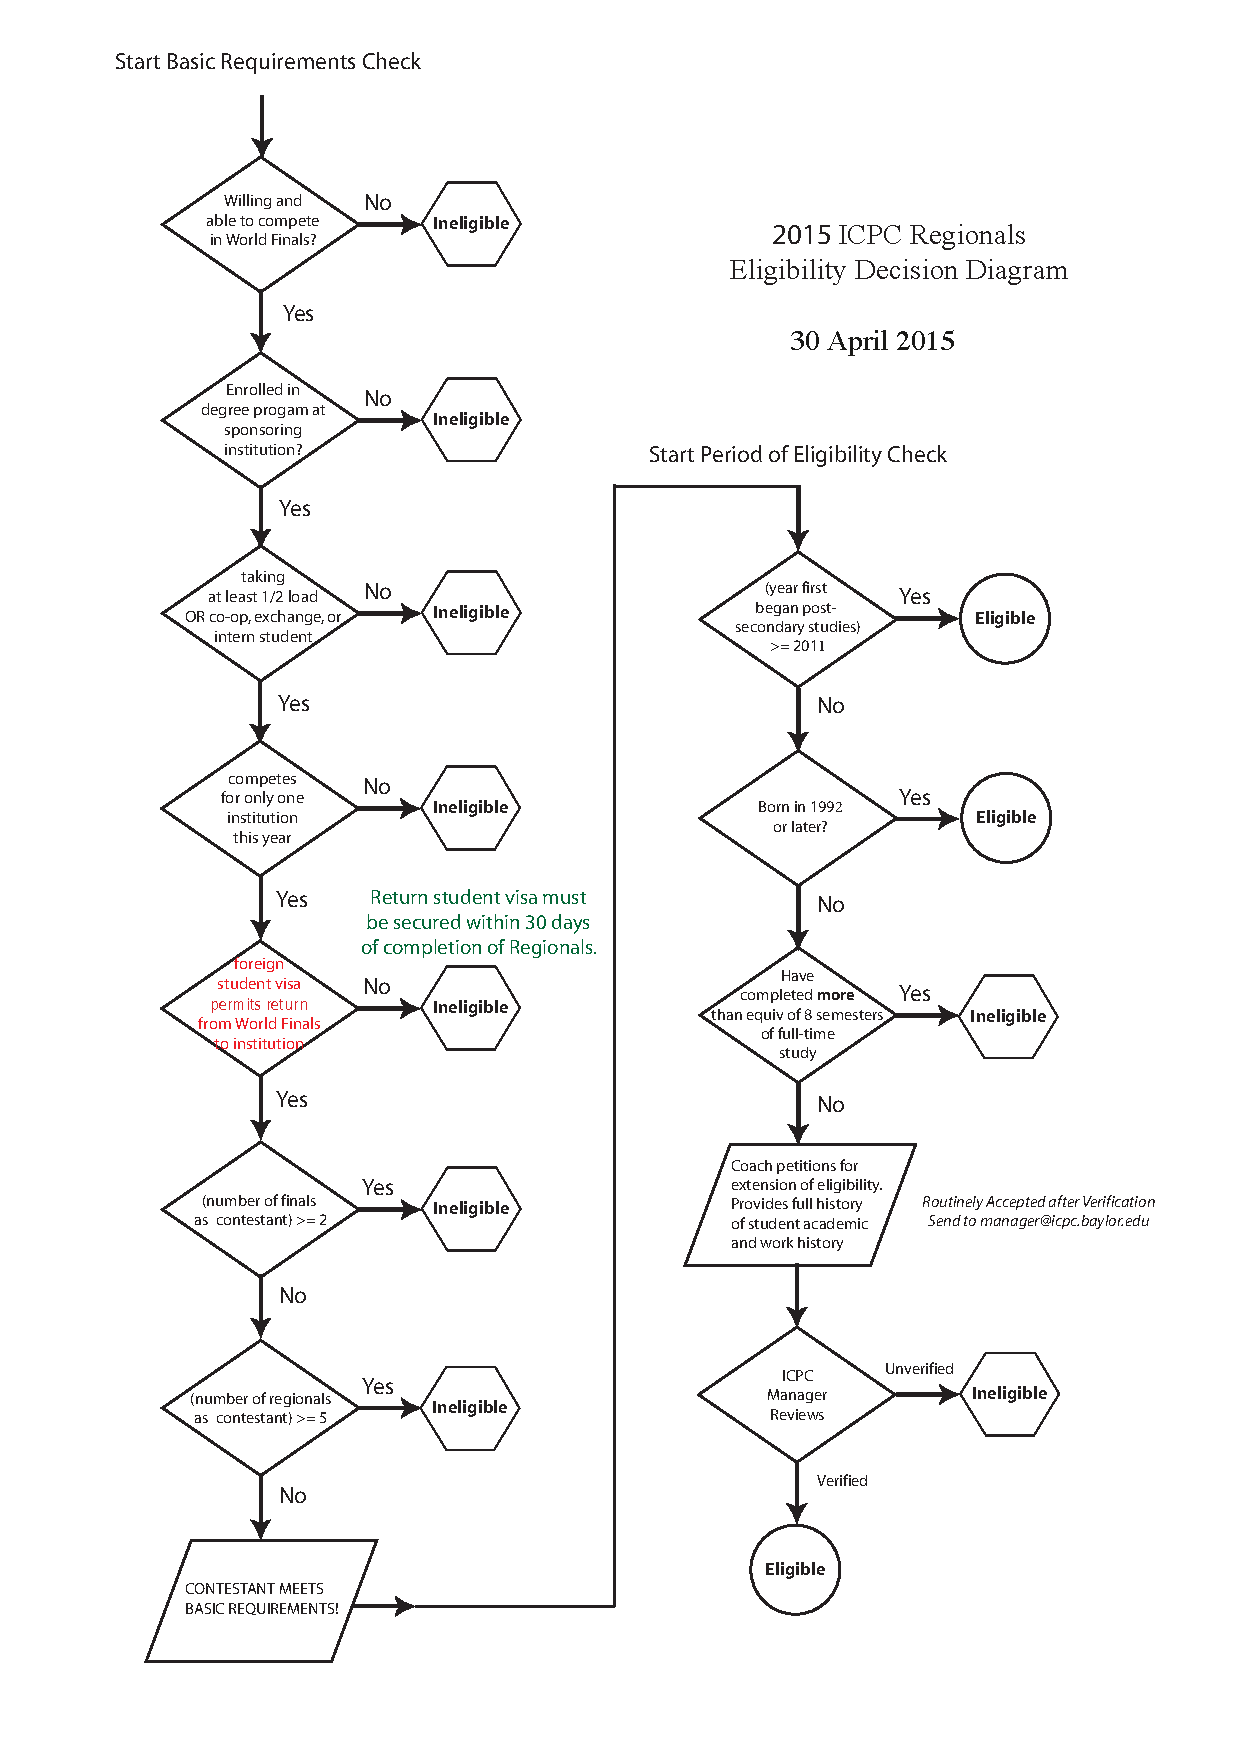
\includepdf[pages=-1]{./Attachments/EligibilityDecisionTree-2015.pdf}

\begin{center}
\vspace*{\fill}
This page is intentionally left blank.
\vspace*{\fill}
\end{center}
\clearpage

\section{DOMjudge team manual}\label{DJteam}
%\addcontentsline{toc}{section}{DOMjudge team manual}
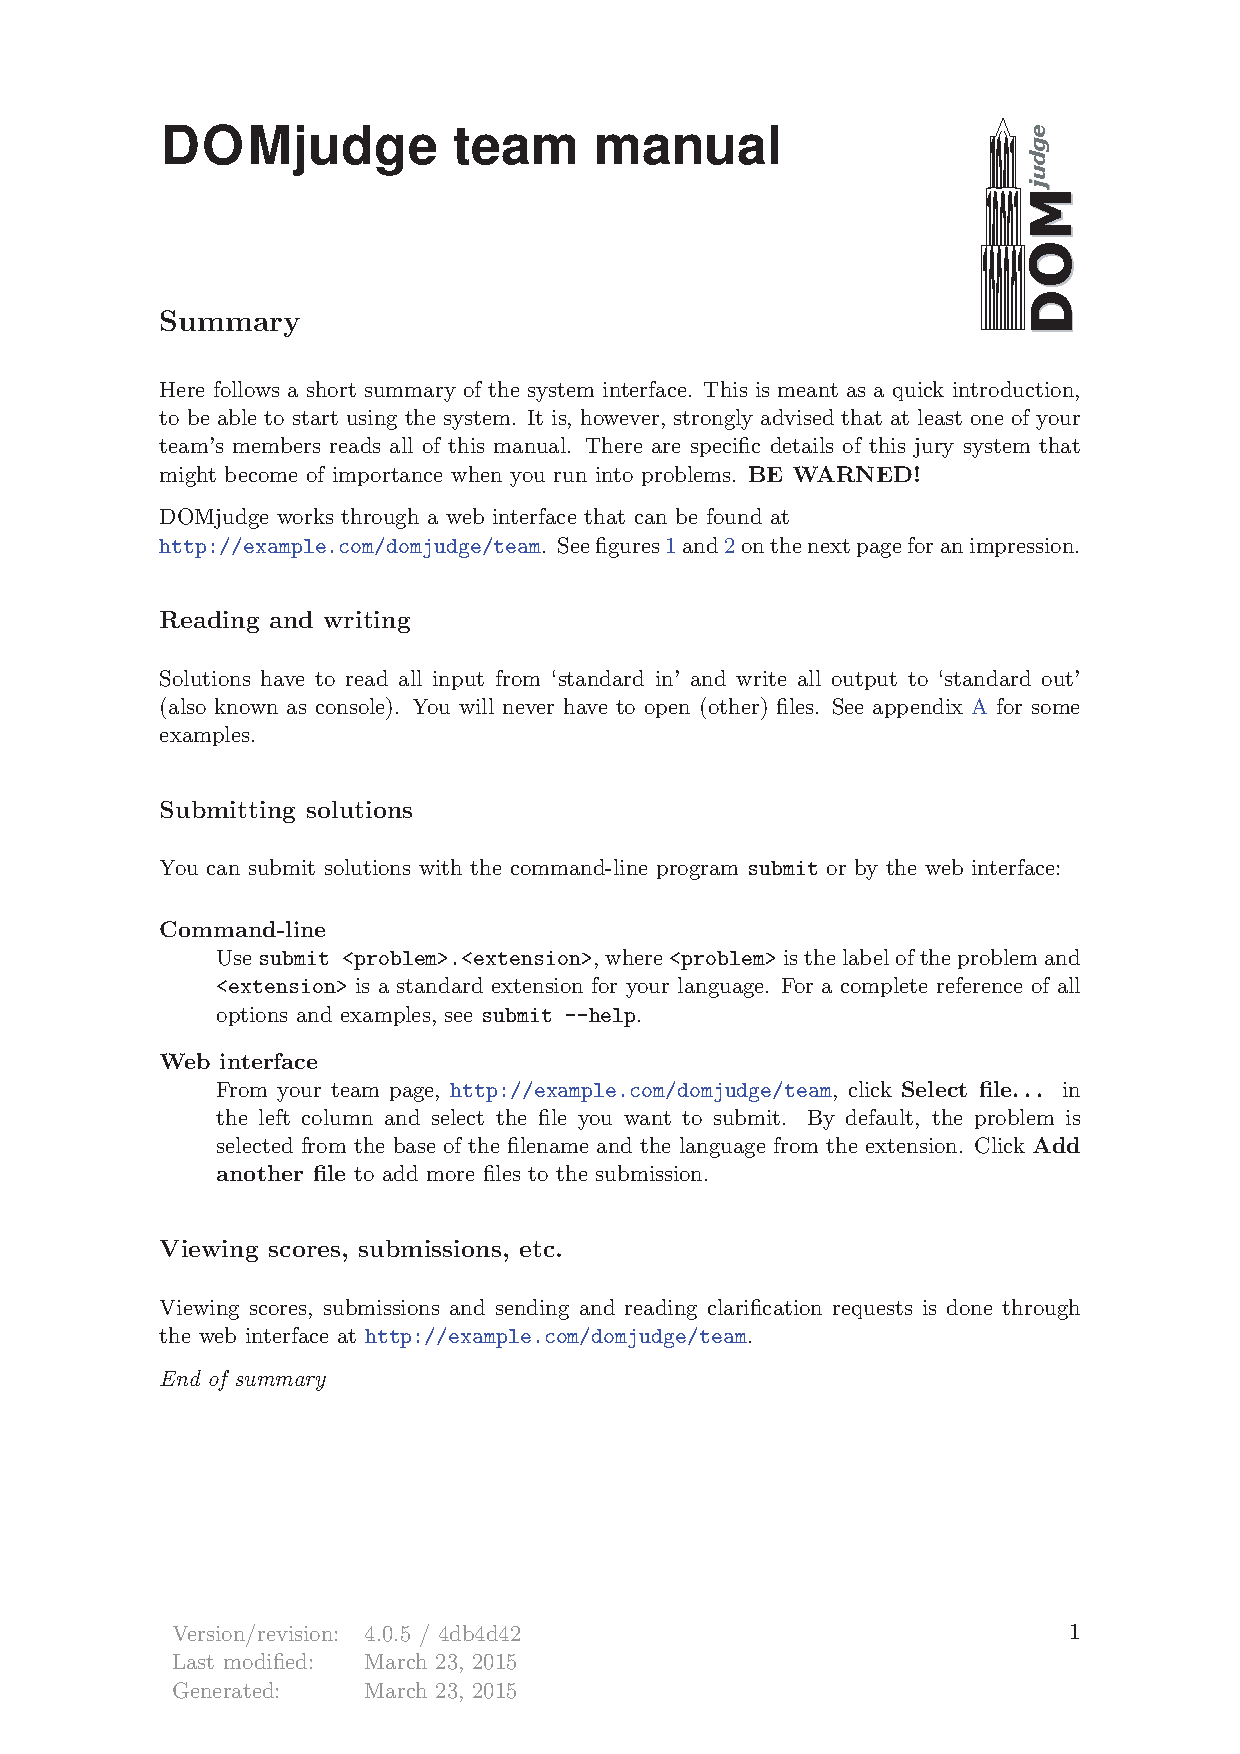
\includepdf[pages=-]{./Attachments/DOMjudge/team-manual.pdf}

\section{Amsterdam Algorithm Programming Preliminaries}\label{Rulebook}

\includepdf[pages=1-3]{./Attachments/Rules/BAPC_Rules_2015.pdf} %pages=- (om alles in te laden van de PDF) geeft errors

\end{document}